\section{Model Exercise 0-1a (01): Bending fracture test}
\label{sec:mex01}
%------------------------------------------------------------------------------
\Authors{Keita Yoshioka, Amir Sattari, Mathias Nest et al.}
%------------------------------------------------------------------------------
\subsection{Experimental set-up}
%------------------------------------------------------------------------------
Model Exercise 1 (ME 1) is concerned with fracture propagation by external loads (i.e. without internal hydraulic force). Experimental data are taken from Three Point Bending (TPB) tests conducted on Rockville Granite samples (cite Tarokh). TPB experiments are performed by applying a load on the top of the samples and the load is adjusted by keeping the rate of the Crack Mouth Opening Displacement (CMOD) fixed at 0.05 $\mu$m/s.
The schematic of TPB is shown in Figure \ref{fig:ME1_TPB_experiment}.
\todo[inline]{[UFZ](KY) Please add Tarokh reference}
\begin{figure}[!ht]
\centering
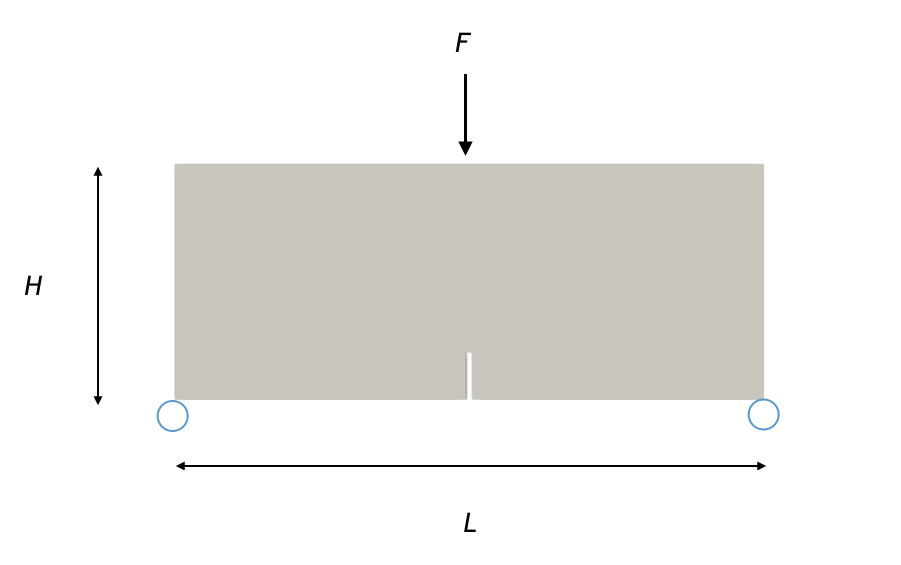
\includegraphics[width=1\textwidth]{figures/TPB_exp.png}
\caption{Three Point Bending experimental set up}
\label{fig:ME1_TPB_experiment}
\end{figure}

The width of the notch is 1.2 mm at the center of the sample and the ratio of notch length to the sample height is 0.2. 
Other parameters used for simulation are listed in Table \ref{table:ME1_TPB_experiment}.

\begin{table}[!ht]
\centering
\begin{tabular}{c c c |c c c c}
$w$ & $L$ (span) & $H$ & $E$ &  $\nu$ &  UCS  & $\sigma_T$  \\
\hline
30 mm & 127 mm & 50.8 mm  & 27.5 GPa & 0.175 & 106 MPa &  8.1 MPa \\
\end{tabular}
\caption{Parameters used for the simulation of Three Point Bending tests. 
\label{table:ME1_TPB_experiment}
}
\label{tabl:Numerical_param_for_sneddon_crack}
\end{table}
The experimental force-displacement results from cite Tarokh for two samples are shown in Figure \ref{fig:ME1_TPB_force_disp}.

\begin{figure}[!ht]
\centering
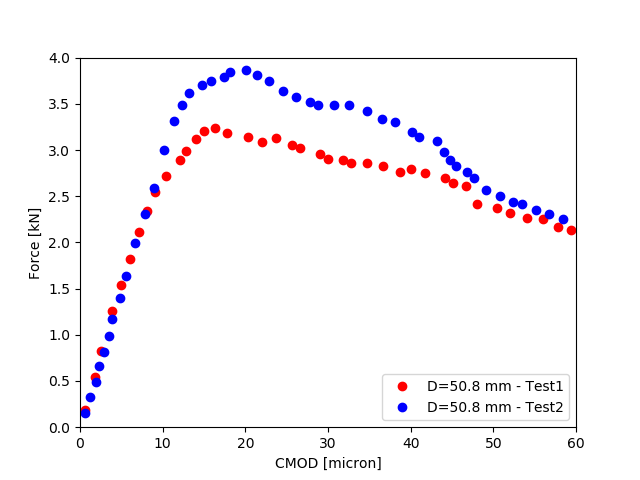
\includegraphics[width=1\textwidth]{figures/TPB_Force_Disp.png}
\caption{Three Point Bending test results.}
\label{fig:ME1_TPB_force_disp}
\end{figure}
%------------------------------------------------------------------------------
\subsection{Model approach}
%------------------------------------------------------------------------------
\subsubsection*{Discrete-Element-Model (DEM)}

Two models were set up to represent granite samples with different grain structures. As reported in reference cite Tarokh, the average grain size of the Rockville granite in the experiment was 10 mm. 
As they are embedded in more finely grained material, a discrete element model with a Voronoi-block diameter of 5.4 mm has been chosen. For the Voronoi-discretization random points were inserted in the sample volume. 
The serve as the center coordinates of the Voronois. After 10$^5$ insertion attempts, this lead to 1236 grains for the first sample, and 1226 for the second sample, see Fig. \ref{fig:ME1_TPB_DEM_domain}. Finally a notch was cut from the models. The behaviour of the model follows from the properties of both the grains (bulk modulus $K$ and shear modulus $G$), and the interface parameters (normal stiffness $k_n$, shear stiffness $k_s$, and tensile strength $\sigma_z$). These can be combined in several ways to reproduce the experimental results in Fig. \ref{fig:ME1_TPB_force_disp}. In this model we have chosen $K$ = 14.1 GPa, $G$ = 11.7 GPa, $k_n$ = 1700 GPa/m, $k_s$ = 170 GPa/m, and $\sigma_z$ = 2.5 MPa. 

\begin{figure}[!ht]
\centering
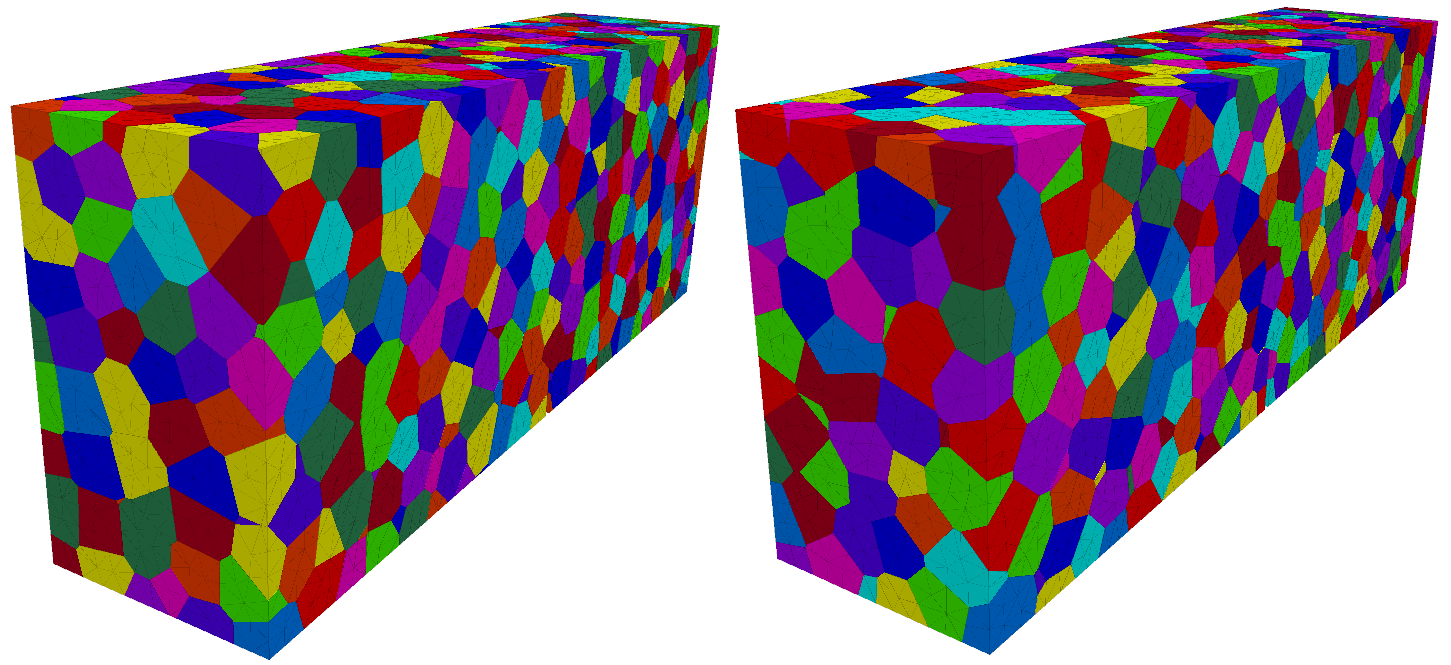
\includegraphics[width=1\textwidth]{figures/ME1-DEM-samples.png}
\caption{Discrete element model computation domain}
\label{fig:ME1_TPB_DEM_domain}
\end{figure}

\subsubsection*{Lattice-Element-Model (LEM)}

The lattice element method (LEM) with the refined mesh is implemented to model the three-point bending test according to the experimental data given in Table \ref{table:ME1_TPB_experiment}. The regularization of the parameters is carried out to assure the mesh independence results (Section \ref{Section:MechanicalLattice}). The total number of the elements is around 500,000 elements, where the distance between the two nodes in the refined boundary is 1.2mm, granting the experimental notch width (Figure \ref{fig:Amir_ME1_LEM_Setup}). The considered Young Modulus is 35GPa to match the experimental linear elastic response.

\begin{figure}[!ht]
\centering
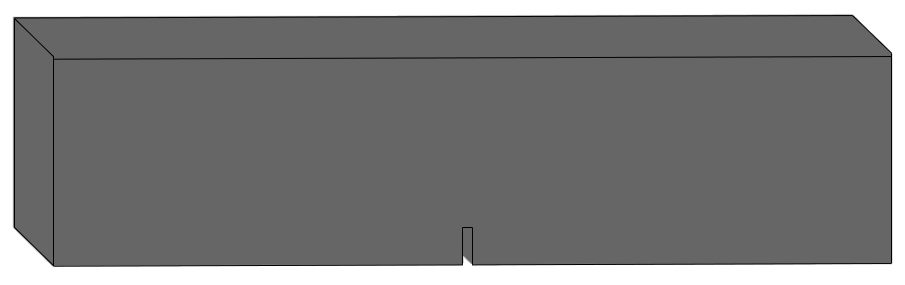
\includegraphics[width=11cm,height=5cm]{figures/Amir_ME1_LEM_Setup.png}
\caption{The lattice setup for the simulation of the fracture toughness}
\label{fig:Amir_ME1_LEM_Setup}
\end{figure}


\subsubsection*{Finite-Element-Model: Variational Phase-Field (VPF)}

The finite element mesh constructed for the 50.8 mm test is shown in Fig.~\ref{fig:ME1_TPB_VF_domain}, which consists of 1,682,308 three dimensional tetrahedral elements with 316,636 nodes.
The notch with the width of 1.2 mm is explicitly meshed in the domain and the top load is applied at the row of the nodes on the top.
The average tetrahedral size is 0.3 mm, which is 1/4 of the notch width, in the refined region.
The Young's modulus in the simulation was increased to 40 GPa from the one listed in Table~\ref{table:ME1_TPB_experiment} in order to match the linear elastic response. 
Another property required in the variational phase-field model is the fracture toughness rather than macroscopic yield strengths as the methodology is based on fracture mechanics.
The fracture toughness, $G_c$ of 35 Pa-m was chosen to match the peak force from the experiment.

\begin{figure}[!ht]
\centering
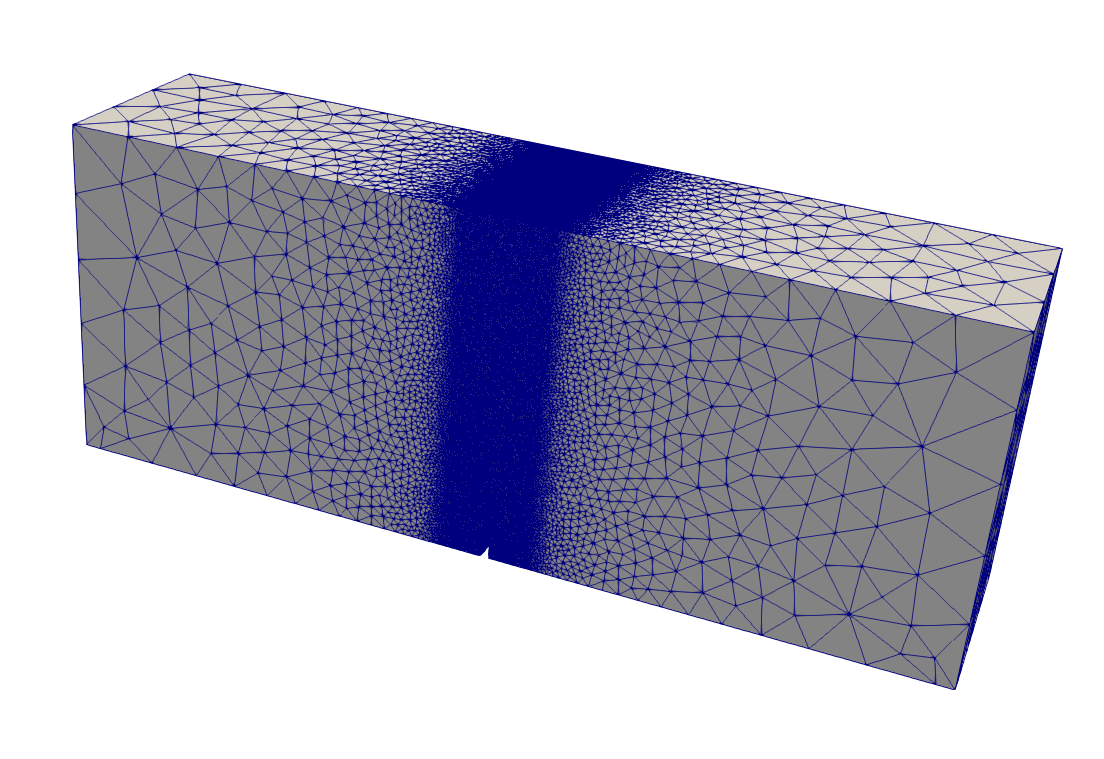
\includegraphics[width=1\textwidth]{figures/VPF_model_domain_mesh.png}
\caption{Variational phase-field computation domain}
\label{fig:ME1_TPB_VF_domain}
\end{figure}

\begin{figure}[!ht]
\centering
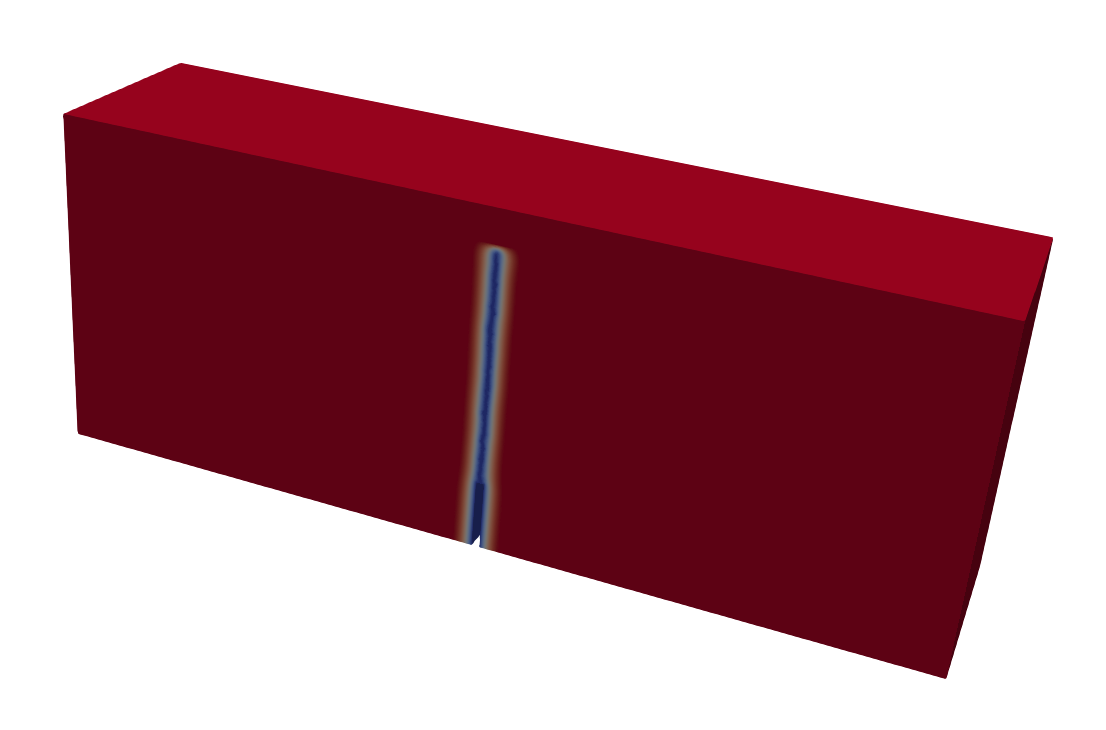
\includegraphics[width=1\textwidth]{figures/VPF_ME1_frac.png}
\caption{Variational phase-field computation result}
\label{fig:ME1_TPB_VPF_result}
\end{figure}

%------------------------------------------------------------------------------
\subsection{Results and discussion}
%------------------------------------------------------------------------------
Simulation results from all the simulations are shown in \ref{fig:ME1_comparison}. 
All the models exhibit linear elastic behaviors, before failure sets in as in the experimental data.
First, we can see that all the models reproduce the linear elastic response.
It is straightforward for the variational phase-field model as it only requires the descriptions of the linear elastic properties (i.e. the Young's modulus and the Poisson's ratio).
However, for the lattice or discrete element methods, these bulk properties need to be obtained through the micro mechanical properties such as (xxx) and they are obtained as.... 
In lattice element method the strain energy stored in unit cell should be equal to the continuum strain energy. Therefore, for a Euler Bernoulli beam elements and while considering 
the stored energies, the micro to macro (bulk) transformation of properties is carried out, see \cite{Ostojastarzewski2002}.

The main difference between the discrete/lattice element method and the variational phase-field model is the responses after the failure.
While the current implementation in the variational phase-field used in this study is based on the linear elastic brittle fracture mechanics, and plasticity or softening is not 
considered \footnote{The linear elastic fracture mechanics formulation is not necessary constrained by the variational phase-field formulation. Models that include ductility, plasticity, 
and softening behaviors exist. For example, see \cite{Alessi2018}}.
For this reason, the result from the variational phase-field model fails elastically and the force ceases to zero quickly after the peak.
On the other hand, the lattice and discrete element methods can model a softening of the bulk material. The implemented softening 
scheme in lattice element is based on bi-linear softening behavior found in \cite{Inceetal2003}.
This post-failure behavior agrees with the real rock response better than the approach based on the linear elastic fracture mechanics.

\begin{figure}[!ht]
\centering
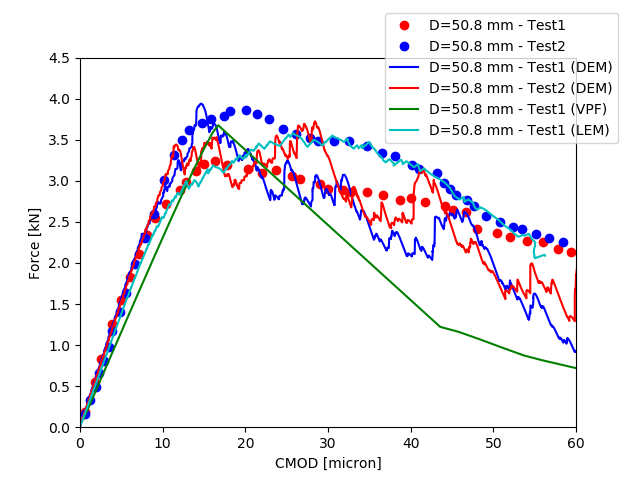
\includegraphics[width=1\textwidth]{figures/ME1_comp_updated.png}
\caption{Model comparison}
\label{fig:ME1_comparison}
\end{figure}

All three methods reproduce a similar pattern of horizontal displacements. The VPF ... The result from the DEM is shown in Fig. \ref{fig:ME1-xdis-dem}. 
The crack does not extend quite as far as in the VPF method, but the absolute extend ... 

\begin{figure}[!ht]
\centering
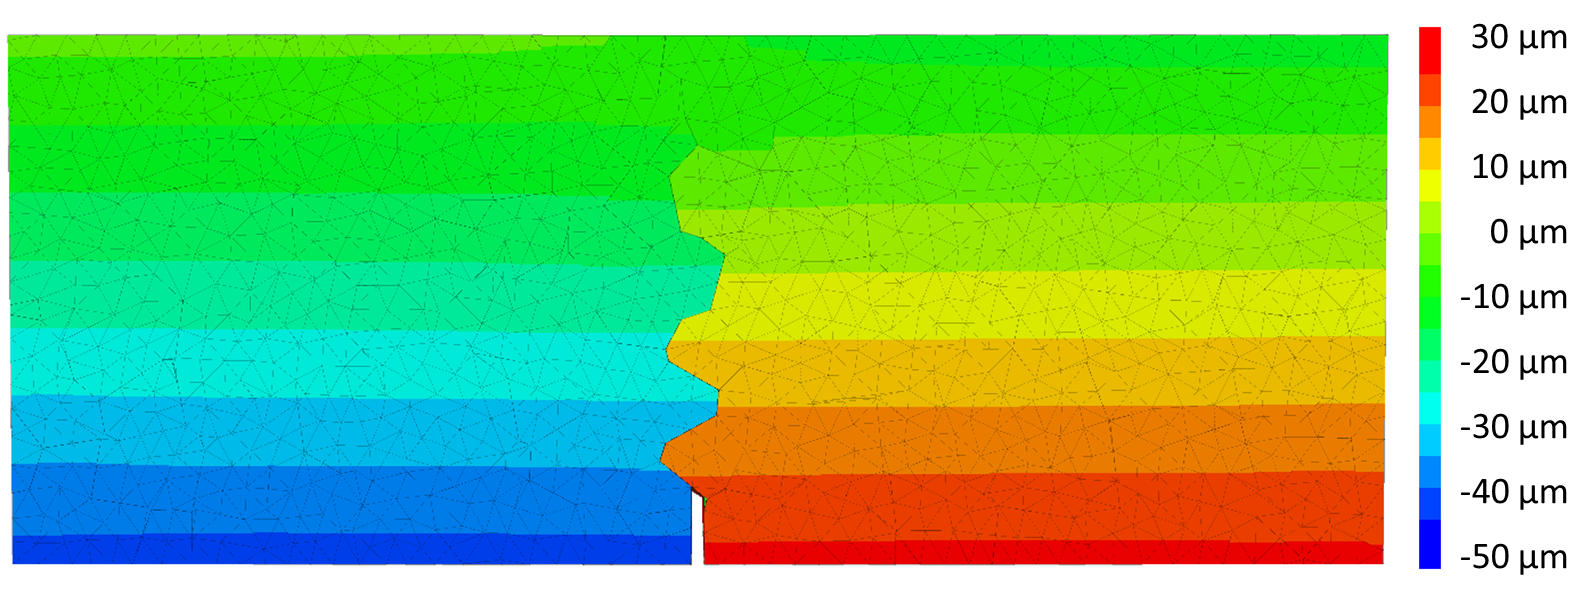
\includegraphics[width=1\textwidth]{figures/ME1-xdis-dem}
\caption{Final Horizontal displacements (DEM)}
\label{fig:ME1-xdis-dem}
\end{figure}

After modeling the crack mouth opening displacement (CMOD) under applied bending load using LEM, the horizontal displacement of the nodes are shown in Figure \ref{fig:Amir_ME1_LEM_Displacement_Crystalline}. The developed crack pattern is visible in mid-section of the simulation, where the neighboring nodes on crack tip are moving in the opposite directions. 

\begin{figure}[!ht]
\centering
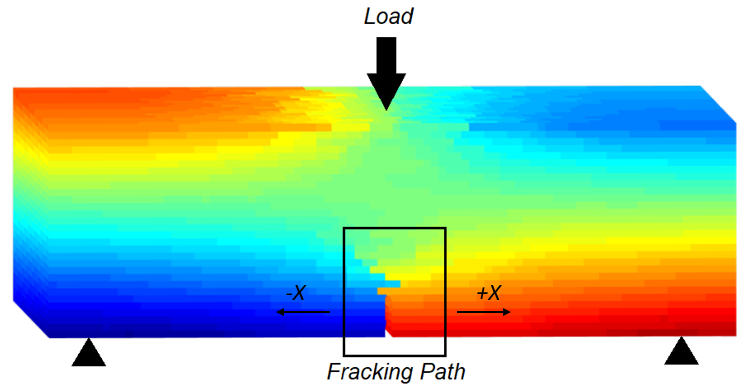
\includegraphics[width=1\textwidth]{figures/Amir_ME1_LEM_Displacement_Crystalline.png}
\caption{The node displacements in X-axis during the fracking process under the applied bending load}
\label{fig:Amir_ME1_LEM_Displacement_Crystalline}
\end{figure}

The article by Tarokh et al. also reports measurements of acoustic emissions, which serve to localize inter-granular micro-cracks. In the DEM method this could be 
reproduced by using the event of tensile contact failures to call a FISH function which writes the location of that contact into a file. The result, the red dots in 
figure \ref{fig:ME1-dem-ae}, agrees very well with the experimental result for the process zone (dashed rectangle).

\begin{figure}[!ht]
\centering
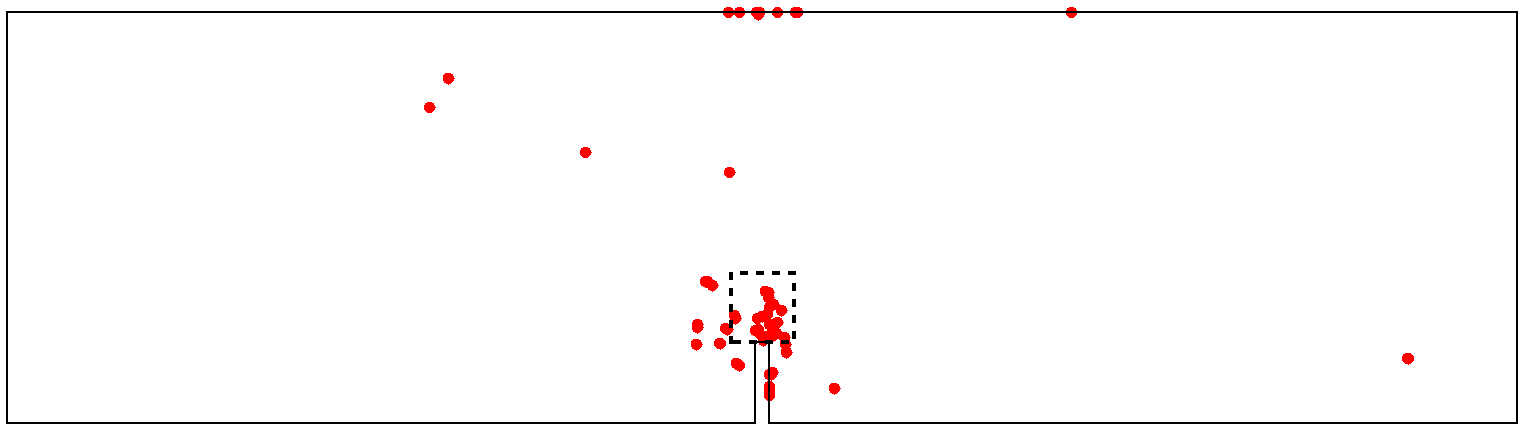
\includegraphics[width=1\textwidth]{figures/sample1-ae-tillmax-v2}
\caption{Locations of acoustic emissions (DEM)}
\label{fig:ME1-dem-ae}
\end{figure}

